\documentclass[12pt,a4paper]{article}

% ─── 1. PACKAGES ──────────────────────────────────────────────────────────────
\usepackage[utf8]{inputenc}
\usepackage[T1]{fontenc}
\usepackage{amsmath, amssymb}
\usepackage{geometry}
\usepackage{graphicx}
\usepackage{xcolor}
\usepackage{listings}
\usepackage{hyperref}
\usepackage{booktabs}
\usepackage{enumitem}
\usepackage{tcolorbox}
\usepackage{mdframed}
\usepackage{fancyhdr}
\usepackage{titlesec}
\usepackage{tikz} 
\usetikzlibrary{shapes.geometric, positioning, arrows.meta, calc, decorations.pathreplacing}

% Font Settings
\usepackage{newtxtext,newtxmath} % Times New Roman
\usepackage{courier}             % Courier New untuk kode

\geometry{margin=2.5cm}

% ─── 2. WARNA TEMA ────────────────────────────────────────────────────────────
\definecolor{codebg}{RGB}{245,247,250}
\definecolor{codeframe}{RGB}{180,195,215}
\definecolor{keywordcolor}{RGB}{0,112,192}
\definecolor{commentcolor}{RGB}{100,160,100}
\definecolor{stringcolor}{RGB}{180,70,50}
\definecolor{notebg}{RGB}{255,249,230}
\definecolor{noteframe}{RGB}{230,180,50}
\definecolor{tipbg}{RGB}{230,245,235}
\definecolor{tipframe}{RGB}{50,160,90}
\definecolor{sectioncolor}{RGB}{30,80,150}

% ─── 3. STYLE SECTION & TOC ───────────────────────────────────────────────────
\titleformat{\section}{\Large\bfseries\color{sectioncolor}}{}{0em}{\thesection\quad}[\titlerule]
\titleformat{\subsection}{\large\bfseries\color{sectioncolor!80}}{}{0em}{\thesubsection\quad}

% Style Table of Contents
\usepackage{tocloft}
\renewcommand{\cftsecleader}{\cftdotfill{\cftdotsep}}
\renewcommand{\cftsecfont}{\bfseries\color{sectioncolor}}

% ─── 4. LISTINGS (CODE STYLE) ─────────────────────────────────────────────────
\lstdefinestyle{customstyle}{
  basicstyle=\ttfamily\small,
  backgroundcolor=\color{codebg},
  frame=single,
  rulecolor=\color{codeframe},
  keywordstyle=\bfseries\color{keywordcolor},
  commentstyle=\itshape\color{commentcolor},
  stringstyle=\color{stringcolor},
  numbers=left,
  numberstyle=\tiny\color{gray},
  breaklines=true,
  tabsize=4,
  showstringspaces=false
}
\lstset{style=customstyle}

% ─── 5. KOTAK CATATAN (MD-FRAME) ──────────────────────────────────────────────
\newmdenv[
  backgroundcolor=notebg, linecolor=noteframe, linewidth=2pt,
  leftline=true, topline=false, rightline=false, bottomline=false,
  innerleftmargin=10pt, innertopmargin=6pt, innerbottommargin=6pt, skipabove=8pt
]{notebox}

\newmdenv[
  backgroundcolor=tipbg, linecolor=tipframe, linewidth=2pt,
  leftline=true, topline=false, rightline=false, bottomline=false,
  innerleftmargin=10pt, innertopmargin=6pt, innerbottommargin=6pt, skipabove=8pt
]{tipbox}

% ─── 6. HEADER & FOOTER ───────────────────────────────────────────────────────
\pagestyle{fancy}
\fancyhf{}
\fancyhead[L]{\small\textit{Rekayasa Perangkat Lunak}}
\fancyhead[R]{\small\textit{noteify -- Model Proses PL}}
\fancyfoot[C]{\thepage}
\renewcommand{\headrulewidth}{0.4pt}

% ─── 7. DATA COVER ────────────────────────────────────────────────────────────
\title{
  {\LARGE\bfseries REKAYASA PERANGKAT LUNAK}\\[0.5em]
  {\large Modul Pembelajaran: Model Proses Perangkat Lunak (SDLC)}\\[0.8em]
  {\normalsize Penjelasan komprehensif mengenai siklus hidup pengembangan perangkat lunak, aktivitas dasar, dan ragam model arsitektur seperti Waterfall, Prototype, RAD, Incremental, hingga Spiral.}
}
\author{}
\date{}

% ==============================================================================
\begin{document}

\maketitle
\thispagestyle{fancy}
\tableofcontents
\newpage

% ─── KONTEN MATERI ─────────────────────────────────────────────────────────────

\section{Pengantar Siklus Hidup Perangkat Lunak}

Membangun sebuah perangkat lunak berskala besar ibarat membangun sebuah gedung pencakar langit. Proses ini tidak bisa sekadar diawali dengan niat lalu langsung menyusun batu bata (menulis kode). Proses rekayasa perangkat lunak melibatkan keseimbangan antara Proses Manajemen Proyek dan Proses Pengembangan Perangkat Lunak itu sendiri.

\subsection{Konsep Model Proses (Paradigma)}
Menurut Ian Sommerville, sebuah model proses atau paradigma rekayasa perangkat lunak menunjukkan suatu strategi untuk melindungi dan mengelola proses, metode, serta alat bantu secara efektif agar dapat mengirimkan produk perangkat lunak dengan sukses. 

Bagaimana cara memilih model proses yang tepat? Pemilihannya didasarkan pada tiga hal utama:
\begin{itemize}
    \item Proyek dan aplikasi yang alami (karakteristik dasar dari aplikasi yang akan dibuat).
    \item Metode dan alat bantu yang digunakan oleh tim.
    \item Kebutuhan akan kontrol dan pengiriman (\textit{delivery}) produk.
\end{itemize}

Terlepas dari model apa yang nantinya dipilih, terdapat empat aktivitas dasar yang pasti ada di setiap proses rekayasa perangkat lunak:
\begin{enumerate}
    \item \textbf{Software specification} (Spesifikasi perangkat lunak).
    \item \textbf{Software development} (Pengembangan perangkat lunak).
    \item \textbf{Software validation} (Validasi atau pengujian perangkat lunak).
    \item \textbf{Software evolution} (Evolusi atau pemeliharaan perangkat lunak).
\end{enumerate}

\subsection{Memahami SDLC (Software Development Life Cycle)}
\textit{Software Development Life Cycle} (SDLC) adalah sebuah pendekatan yang disiplin dan sistematis dalam membagi proses pengembangan perangkat lunak ke dalam berbagai fase yang terstruktur, seperti fase kebutuhan (\textit{requirement}), perancangan (\textit{design}), dan pengkodean (\textit{coding}). 

Tujuan utama dari penerapan fase-fase SDLC ini adalah untuk membantu manajer dan pengembang melacak jadwal (\textit{schedule}), biaya (\textit{cost}), dan kualitas dari proyek perangkat lunak tersebut.

Secara rinci, terdapat enam fase utama dalam sebuah SDLC:
\begin{enumerate}
    \item \textbf{Feasibility analysis phase:} Meliputi analisis kelayakan dan kebutuhan proyek.
    \item \textbf{Requirement analysis and specification phase:} Meliputi proses pengumpulan (\textit{gathering}), menganalisis, memvalidasi, dan menspesifikasikan kebutuhan sistem ke dalam dokumen SRS (\textit{Software Requirement Specification}).
    \item \textbf{Design phase:} Meliputi proses penerjemahan kebutuhan yang dispesifikasikan di SRS menjadi struktur logis yang nantinya dapat diimplementasikan ke dalam bahasa pemrograman.
    \item \textbf{Coding phase:} Meliputi implementasi desain (dari dokumen desain) menjadi kode eksekusi menggunakan bahasa pemrograman tertentu.
    \item \textbf{Testing phase:} Meliputi pencarian dan pendeteksian \textit{error} (kesalahan) di dalam perangkat lunak.
    \item \textbf{Maintenance phase:} Meliputi penerapan perubahan dan penambahan kebutuhan baru pada perangkat lunak di lokasi pengguna/pelanggan (\textit{customer location}).
\end{enumerate}

\newpage
\section{1. Model Sekuensial Linier (Waterfall)}

Model proses perangkat lunak yang paling klasik dan paling mudah dipahami adalah Model \textbf{Waterfall} (Air Terjun). Disebut air terjun karena aliran prosesnya mengalir ke bawah secara linier dan berurutan dari satu tahap ke tahap selanjutnya.

\begin{figure}[h]
    \centering
    \resizebox{\textwidth}{!}{%
    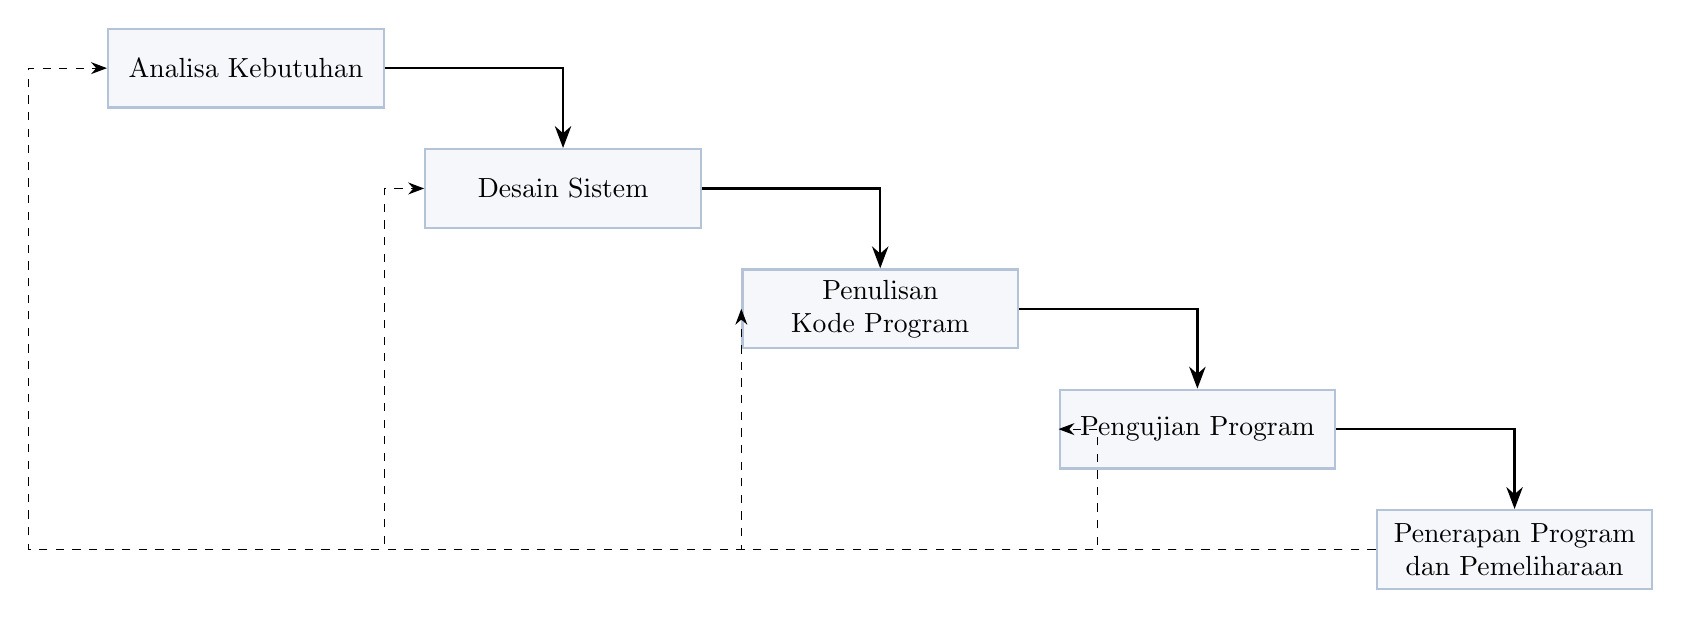
\begin{tikzpicture}[
        node distance=0.5cm and 0.5cm,
        box/.style={draw, rectangle, minimum width=3.5cm, minimum height=1cm, align=center, fill=codebg, draw=codeframe, thick},
        arr/.style={-{Stealth[scale=1.2]}, thick}
    ]
    
    \node[box] (req) {Analisa Kebutuhan};
    \node[box] (des) [below right=of req] {Desain Sistem};
    \node[box] (code) [below right=of des] {Penulisan\\Kode Program};
    \node[box] (test) [below right=of code] {Pengujian Program};
    \node[box] (maint) [below right=of test] {Penerapan Program\\dan Pemeliharaan};

    % Connecting arrows
    \draw[arr] (req.east) -| (des.north);
    \draw[arr] (des.east) -| (code.north);
    \draw[arr] (code.east) -| (test.north);
    \draw[arr] (test.east) -| (maint.north);

    % Backwards arrows (maintenance loops)
    \draw[-{Stealth[scale=1.2]}, dashed] (maint.west) -| ([xshift=-1cm]req.west) |- (req.west);
    \draw[-{Stealth[scale=1.2]}, dashed] (maint.west) -| ([xshift=-0.5cm]des.west) |- (des.west);
    \draw[-{Stealth[scale=1.2]}, dashed] (maint.west) -| (code.west);
    \draw[-{Stealth[scale=1.2]}, dashed] (maint.west) -| ([xshift=0.5cm]test.west) |- (test.west);

    \end{tikzpicture}%
    }
    \caption{Skema Aliran Model Waterfall.}
\end{figure}

\subsection{Evaluasi Model Waterfall}
Model ini mengunci setiap fase sebelum lanjut ke fase berikutnya. Berikut adalah karakteristik keunggulannya:
\begin{itemize}
    \item \textbf{Kualitas Tinggi:} Kualitas dari sistem yang dihasilkan akan sangat baik karena setiap langkah diuji dan diselesaikan secara tuntas.
    \item \textbf{Dokumentasi Terorganisir:} Dokumen pengembangan sistem menjadi sangat rapi dan terorganisir.
    \item \textbf{Kepastian Kebutuhan:} Sangat cocok digunakan jika kebutuhan aplikasi sudah diketahui dengan baik dari awal proyek.
\end{itemize}

Namun, karena sifatnya yang kaku, model ini memiliki beberapa kelemahan fatal:
\begin{itemize}
    \item \textbf{Efek Domino Kesalahan:} Kesalahan kecil di awal akan menjadi masalah yang sangat besar jika tidak segera diketahui sejak awal.
    \item \textbf{Kendala Pelanggan:} Pelanggan seringkali sulit untuk menyatakan dan membayangkan kebutuhannya secara eksplisit di awal proyek.
    \item \textbf{Waktu Tidak Efisien:} Proses pengembangan harus menunggu tahap sebelumnya selesai baru bisa lanjut ke tahap berikutnya, sehingga banyak waktu tunggu (\textit{idle}).
\end{itemize}

\newpage
\section{2. Model Prototipe (Prototyping)}

Menjawab kelemahan Waterfall di mana pelanggan sulit membayangkan kebutuhan di awal, hadirlah Model Prototipe. Model ini berfungsi sebagai mekanisme untuk mengidentifikasi kebutuhan perangkat lunak di awal dengan cepat. Melalui "Perancangan Kilat", model ini menyajikan gambaran aspek perangkat lunak yang kemudian digunakan untuk menyaring dan memvalidasi kebutuhan pelanggan.

\begin{figure}[h]
    \centering
    \resizebox{0.85\textwidth}{!}{%
    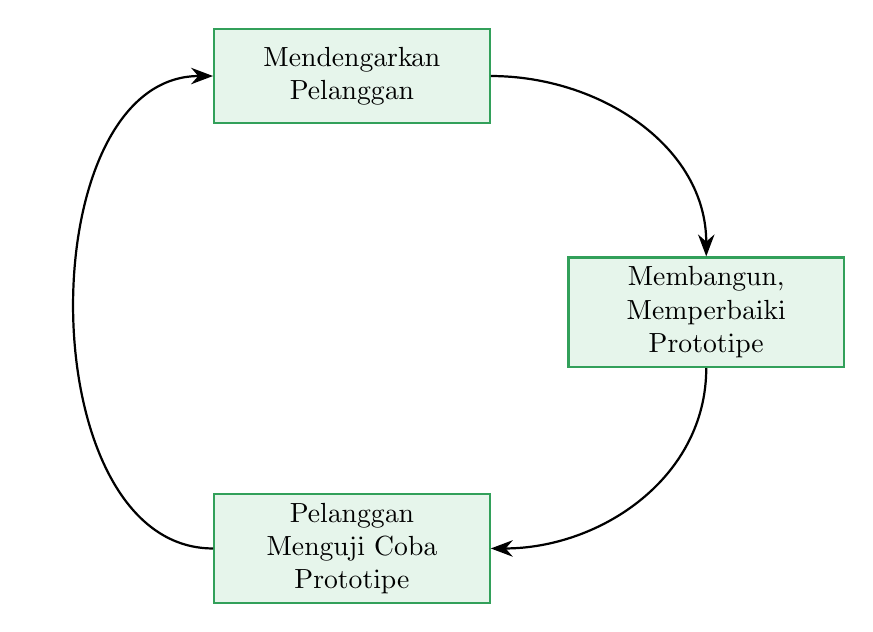
\begin{tikzpicture}[
        box/.style={draw, rectangle, minimum width=3.5cm, minimum height=1.2cm, align=center, fill=tipbg, draw=tipframe, thick},
        arr/.style={-{Stealth[scale=1.2]}, thick}
    ]
    
    \node[box] (listen) at (0, 3) {Mendengarkan\\Pelanggan};
    \node[box] (build) at (4.5, 0) {Membangun,\\Memperbaiki\\Prototipe};
    \node[box] (test) at (0, -3) {Pelanggan\\Menguji Coba\\Prototipe};

    \draw[arr] (listen) to[out=0,in=90, looseness=1] (build);
    \draw[arr] (build) to[out=270,in=0, looseness=1] (test);
    \draw[arr] (test) to[out=180,in=180, looseness=1] (listen);

    \end{tikzpicture}%
    }
    \caption{Siklus Berulang pada Model Prototipe.}
\end{figure}

\subsection{Evaluasi Model Prototipe}
Keunggulan dari model Prototipe adalah pendekatan interaktifnya:
\begin{itemize}
    \item Terdapat \textbf{komunikasi yang baik} antara pengembang dan pelanggan.
    \item Pengembang dapat bekerja lebih baik dan tepat sasaran.
    \item Pelanggan \textbf{berperan sangat aktif} selama proses pengembangan sistem.
\end{itemize}

Namun, model ini juga menyimpan jebakan (risiko) yang sering membuat kualitas akhir perangkat lunak menurun:
\begin{itemize}
    \item Pelanggan terkadang tidak paham bahwa prototipe perangkat lunak yang ada belum mencantumkan standar kualitas dan pemeliharaan untuk jangka waktu yang lama.
    \item Pengembang biasanya ingin cepat-cepat menyelesaikan proyek, sehingga mereka menggunakan algoritma dan bahasa pemrograman yang sederhana agar lebih cepat selesai. Padahal, mereka melakukan itu tanpa memikirkan bahwa program prototipe tersebut akan menjadi \textit{blue print} sistem ke depannya.
\end{itemize}

\newpage
\section{3. Rapid Application Development (RAD)}

Model \textbf{Rapid Application Development (RAD)} adalah model yang sangat mengedepankan kecepatan. RAD menekankan siklus pengembangan yang sangat pendek, biasanya ditekan hingga selesai dalam \textbf{60-90 hari} saja! Pengembangan yang sangat cepat ini dicapai melalui pendekatan konstruksi berbasis komponen, di mana beberapa tim dipecah secara paralel.

\begin{figure}[h]
    \centering
    \resizebox{\textwidth}{!}{%
    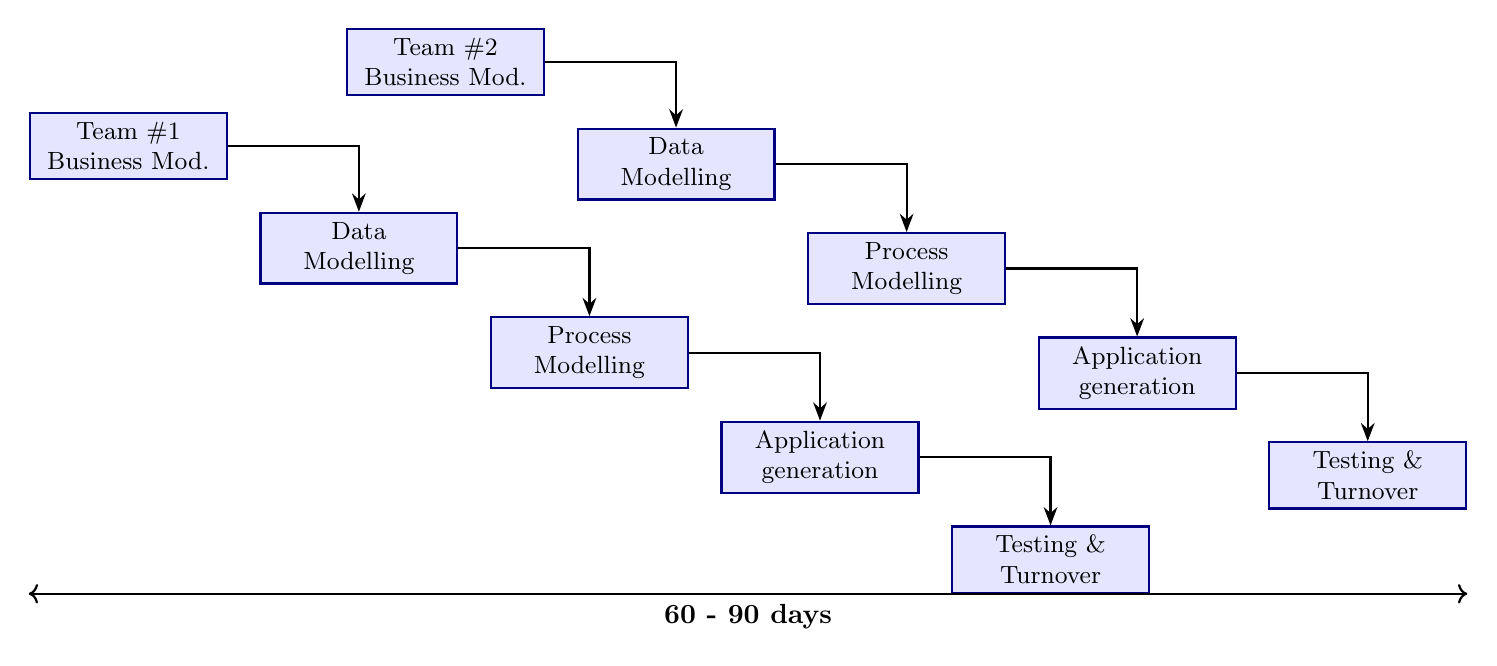
\begin{tikzpicture}[
        node distance=0.4cm and 0.4cm,
        box/.style={draw, rectangle, minimum width=2.5cm, minimum height=0.8cm, align=center, fill=blue!10, draw=blue!50!black, thick, font=\small},
        arr/.style={-{Stealth[scale=1]}, thick}
    ]
    
    % Team 1
    \node[box] (b1) {Team \#1\\Business Mod.};
    \node[box] (d1) [below right=of b1] {Data\\Modelling};
    \node[box] (p1) [below right=of d1] {Process\\Modelling};
    \node[box] (a1) [below right=of p1] {Application\\generation};
    \node[box] (t1) [below right=of a1] {Testing \&\\Turnover};
    
    \draw[arr] (b1.east) -| (d1.north); \draw[arr] (d1.east) -| (p1.north); 
    \draw[arr] (p1.east) -| (a1.north); \draw[arr] (a1.east) -| (t1.north);

    % Team 2 (shifted up and right)
    \node[box] (b2) [above right=0.2cm and 1.5cm of b1] {Team \#2\\Business Mod.};
    \node[box] (d2) [below right=of b2] {Data\\Modelling};
    \node[box] (p2) [below right=of d2] {Process\\Modelling};
    \node[box] (a2) [below right=of p2] {Application\\generation};
    \node[box] (t2) [below right=of a2] {Testing \&\\Turnover};

    \draw[arr] (b2.east) -| (d2.north); \draw[arr] (d2.east) -| (p2.north); 
    \draw[arr] (p2.east) -| (a2.north); \draw[arr] (a2.east) -| (t2.north);
    
    % Timeline arrow
    \draw[<->, thick] (b1.west |- t1.south) -- (t2.east |- t1.south) node[midway, below] {\textbf{60 - 90 days}};

    \end{tikzpicture}%
    }
    \caption{Skema Tim Paralel pada Model RAD.}
\end{figure}

\subsection{Evaluasi Model RAD}
Karena sifatnya yang cepat, RAD memiliki keunggulan tersendiri:
\begin{itemize}
    \item Lebih fleksibel karena pengembang dapat melakukan proses desain ulang pada saat yang bersamaan.
    \item Bisa mengurangi penulisan kode yang kompleks dengan menggunakan komponen siap pakai.
    \item Tampilan yang dihasilkan lebih standar dan nyaman berkat bantuan \textit{software-software} pendukung dalam pembuatannya.
\end{itemize}

Namun, risiko dari memaksakan kecepatan adalah kualitas yang sering dikorbankan:
\begin{itemize}
    \item Lebih banyak terjadi kesalahan apabila tim hanya mengutamakan kecepatan pembuatan.
    \item Fasilitas-fasilitas banyak yang terpaksa dikurangi karena terbatasnya waktu yang tersedia.
    \item Sistem yang dihasilkan menjadi sulit untuk diaplikasikan di tempat yang lain.
    \item Fasilitas yang sebenarnya tidak perlu terkadang harus disertakan secara paksa, karena tim menggunakan komponen yang sudah jadi (\textit{drag-and-drop}).
\end{itemize}

\begin{tipbox}
\textbf{Modifikasi Modern dari RAD: Agile Software} \\
Konsep kecepatan RAD berevolusi menjadi pendekatan \textbf{Agile Software}. Agile menekankan interaksi pengembang dengan pelanggan yang bertujuan membangun perangkat lunak yang tangkas dalam menghadapi perubahan. 
Beberapa macam turunan Agile antara lain:
\begin{enumerate}
    \item \textbf{Scrum:} Membagi pekerjaan ke dalam tim-tim yang saling bekerja secara \textit{overlap} (tumpang tindih).
    \item \textbf{Extreme Programming (XP):} Mengutamakan intensitas komunikasi yang sangat sering antara pengembang dan pelanggan.
\end{enumerate}
\end{tipbox}

\newpage
\section{4. Model Evolusioner Inkremental}

Model \textbf{Inkremental} adalah perpaduan jenius yang menggabungkan elemen-elemen dari model sekuensial linier (Waterfall) yang diimplementasikan secara berulang, dengan filosofi dari model \textit{prototype} iteratif.
Setiap iterasi akan menghasilkan sebuah "Inkremen" (potongan modul aplikasi yang bisa langsung berfungsi).

\begin{figure}[h]
    \centering
    \resizebox{\textwidth}{!}{%
    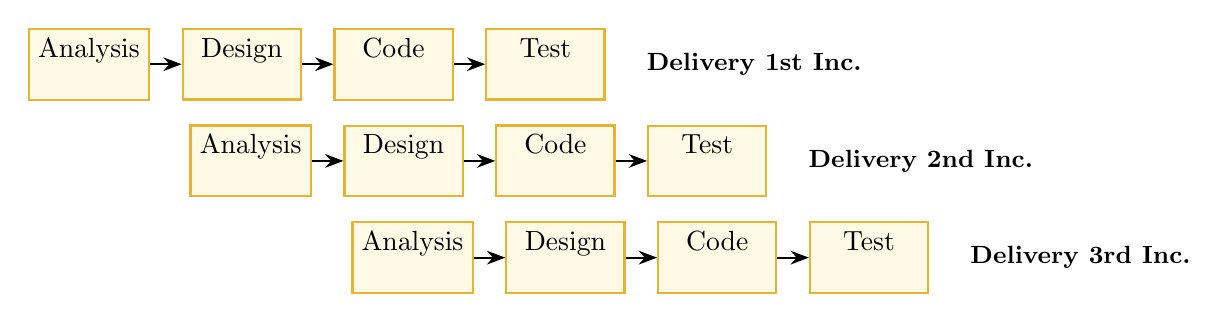
\begin{tikzpicture}[
        node distance=0.4cm and 0.4cm,
        box/.style={draw, rectangle, minimum width=1.5cm, minimum height=0.6cm, align=center, fill=notebg, draw=noteframe, thick},
        arr/.style={-{Stealth[scale=1]}, thick}
    ]
    
    % Increment 1
    \node[box] (a1) {Analysis\\ \textnormal{}};
    \node[box] (d1) [right=of a1] {Design\\ \textnormal{}};
    \node[box] (c1) [right=of d1] {Code\\ \textnormal{}};
    \node[box] (t1) [right=of c1] {Test\\ \textnormal{}};
    \node[right=of t1, font=\small\bfseries] {Delivery 1st Inc.};
    \draw[arr] (a1) -- (d1); \draw[arr] (d1) -- (c1); \draw[arr] (c1) -- (t1);

    % Increment 2
    \node[box] (a2) [below right=0.3cm and 0.5cm of a1] {Analysis\\ \textnormal{}};
    \node[box] (d2) [right=of a2] {Design\\ \textnormal{}};
    \node[box] (c2) [right=of d2] {Code\\ \textnormal{}};
    \node[box] (t2) [right=of c2] {Test\\ \textnormal{}};
    \node[right=of t2, font=\small\bfseries] {Delivery 2nd Inc.};
    \draw[arr] (a2) -- (d2); \draw[arr] (d2) -- (c2); \draw[arr] (c2) -- (t2);

    % Increment 3
    \node[box] (a3) [below right=0.3cm and 0.5cm of a2] {Analysis\\ \textnormal{}};
    \node[box] (d3) [right=of a3] {Design\\ \textnormal{}};
    \node[box] (c3) [right=of d3] {Code\\ \textnormal{}};
    \node[box] (t3) [right=of c3] {Test\\ \textnormal{}};
    \node[right=of t3, font=\small\bfseries] {Delivery 3rd Inc.};
    \draw[arr] (a3) -- (d3); \draw[arr] (d3) -- (c3); \draw[arr] (c3) -- (t3);

    \end{tikzpicture}%
    }
    \caption{Pengembangan Bertahap pada Model Inkremental.}
\end{figure}

\subsection{Evaluasi Model Inkremental}
Pendekatan cicilan fungsionalitas ini memberi nilai lebih:
\begin{itemize}
    \item Pelanggan \textbf{tidak perlu menunggu sampai seluruh sistem selesai} dikirimkan untuk mulai mengambil keuntungan dari fungsionalitas sistem tersebut.
    \item \textbf{Risiko untuk kegagalan proyek secara keseluruhan lebih rendah}, karena setiap modul dikembangkan dan dievaluasi secara berkala.
\end{itemize}

Namun, memecah sistem juga memiliki tantangan tersendiri:
\begin{itemize}
    \item Inkremen yang dibuat harus relatif lebih kecil (patokannya tidak boleh lebih dari 20.000 baris kode).
    \item Setiap inkremen harus dipastikan bisa menyediakan sebagian dari fungsional utuh sistem.
    \item Terdapat kesulitan untuk memetakan spesifikasi persyaratan pelanggan ke dalam potongan-potongan inkremen dengan ukuran yang benar-benar pas.
\end{itemize}

\newpage
\section{5. Model Evolusioner Spiral}

Model terakhir dan yang paling tangguh untuk proyek raksasa adalah \textbf{Model Evolusioner Spiral}. Model ini merangkai dua sifat sekaligus: pendekatan metode iteratif (berulang) dengan kontrol yang ketat dan aspek sistematis khas dari model sekuensial linear (Waterfall).

Proses bergerak secara spiral dari pusat ke luar, melewati empat kuadran aktivitas secara berulang:
\begin{enumerate}
    \item \textbf{Perencanaan (Komunikasi Pelanggan):} Memahami tujuan, alternatif, dan batasan (\textit{Determine objectives, alternatives and constraints}).
    \item \textbf{Analisis Risiko:} Mengevaluasi setiap alternatif yang ada, serta mengidentifikasi dan menyelesaikan risiko yang terdeteksi (\textit{Evaluate alternatives, identify, resolve risks}).
    \item \textbf{Rekayasa (Konstruksi):} Melakukan tahapan desain, pengkodean, dan pengujian secara sistematis (\textit{Design, Code, Test}).
    \item \textbf{Evaluasi Pelanggan (Peluncuran):} Melibatkan evaluasi dari pelanggan dan merencanakan fase putaran spiral berikutnya (\textit{Review, Plan next phase}).
\end{enumerate}

\begin{figure}[h]
    \centering
    \resizebox{0.85\textwidth}{!}{%
    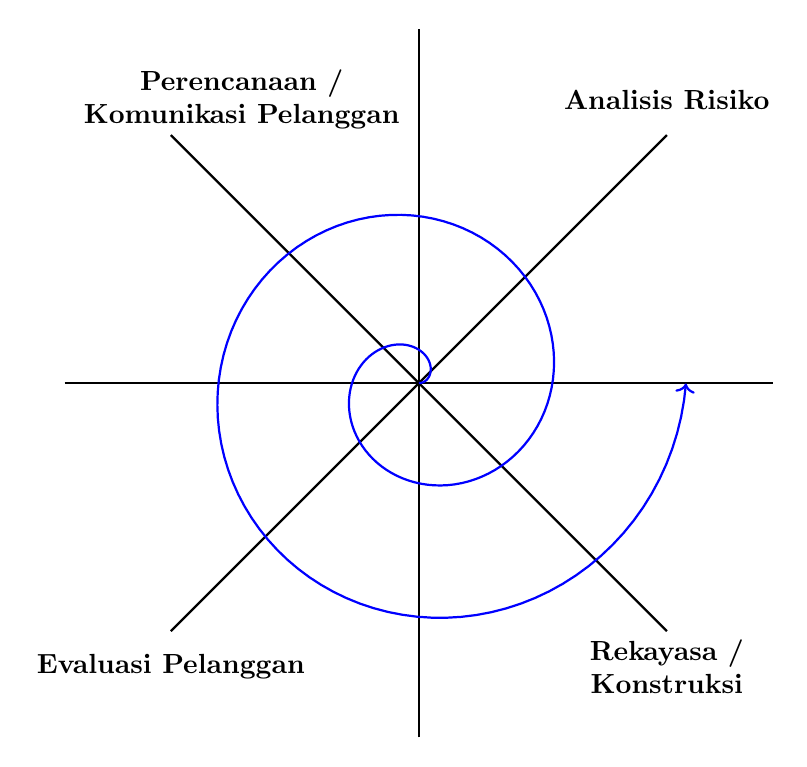
\begin{tikzpicture}[scale=0.9]
        % The quadrants
        \draw[thick] (-5,0) -- (5,0);
        \draw[thick] (0,-5) -- (0,5);
        \draw[thick] (-3.5,-3.5) -- (3.5,3.5);
        \draw[thick] (-3.5,3.5) -- (3.5,-3.5);
        
        % Labels for quadrants
        \node[font=\bfseries, align=center] at (-2.5, 4) {Perencanaan /\\Komunikasi Pelanggan};
        \node[font=\bfseries, align=center] at (3.5, 4) {Analisis Risiko};
        \node[font=\bfseries, align=center] at (3.5, -4) {Rekayasa /\\Konstruksi};
        \node[font=\bfseries, align=center] at (-3.5, -4) {Evaluasi Pelanggan};
        
        % The spiral
        \draw[thick, blue, ->] plot[domain=0:4*pi, variable=\t, samples=200] ({\t r}: {0.3*\t});
    \end{tikzpicture}%
    }
    \caption{Representasi 4 Kuadran pada Model Spiral.}
\end{figure}

\subsection{Evaluasi Model Spiral}
Keunggulan utama dari model Spiral terletak pada manajemen risikonya:
\begin{itemize}
    \item Model ini sangat baik dan disarankan untuk digunakan pada sistem dan \textit{software} berskala besar.
    \item Adanya fase Analisa Risiko pada mekanisme ini dapat memperkecil risiko kegagalan yang fatal.
    \item Adanya kegiatan \textit{prototyping} di dalam putaran spiral akan sangat memudahkan komunikasi teknis dengan konsumen.
\end{itemize}

Sebagai penyeimbang, kelemahan dari model super aman ini adalah:
\begin{itemize}
    \item Memerlukan \textbf{waktu yang cukup lama} (dan biaya besar) untuk mengembangkan \textit{software} karena harus melewati putaran evaluasi dan analisis risiko berulang kali.
    \item Sistem pengendaliannya dinilai kurang baik (karena kompleksitas perputaran iteratif yang harus ditangani manajer proyek).
\end{itemize}

\end{document}